\chapter[head={AI-Agents}, tocentry={Artificial Intelligence Agents}, reference={Artificial Intelligence Agents}]{AI-Agents}\label{sec:ai_agents}
For the experimental evaluation in section \ref{sec:exev}, six different agents were used. The agents can be divided into 2 categories, reinforcement learning (RL) and evolutionary algorithms (EA) agents. The aim of this section is to explain the methods and techniques that are used by the agents. However, the explanations only cover the most important components, due to time and space limitations.

\section{Reinforcement Learning} \label{sec:rl}

Machine Learning (ML) is a sub-field of Artificial Intelligence that is concerned with algorithms that learn from experience \cite[p. 1]{mohri2018foundations}. ML can be divided into 3 paradigms, Supervised Learning, Unsupervised Learning and Reinforcement Learning (RL). In Supervised Learning methods the learner learns from labeled training data, whereas in Unsupervised Learning methods, the learner aims to exploit structure in data without any supervision. Reinforcement Learning is a third paradigm that learns from a \textit{reward signal} that is obtained by interacting in a trial and error manner with an environment. Specifically, it learns by observing a \textit{state} in an \textit{environment}, performing an \textit{action} based on that state and receiving a new state and a reward. This process is known as the agent-environment loop and illustrated in figure \ref{fig:rl_interaction}.

The goal of the agent is to maximize the expected cumulative reward it receives in the long run. This process, or \textit{episode}, repeats until a termination condition is reached. The agent does not know upfront, which action will lead to the highest reward, therefore it has to learn by trial-and-error search and explore which actions lead to high reward. Depending on the environment, the actions might not only affect the immediate reward. They also may lead to distant future rewards by affecting the subsequent states of the environment \cite[pp. 1-2]{richardsutton2018}. 
\begin{figure}[H]%
\centering
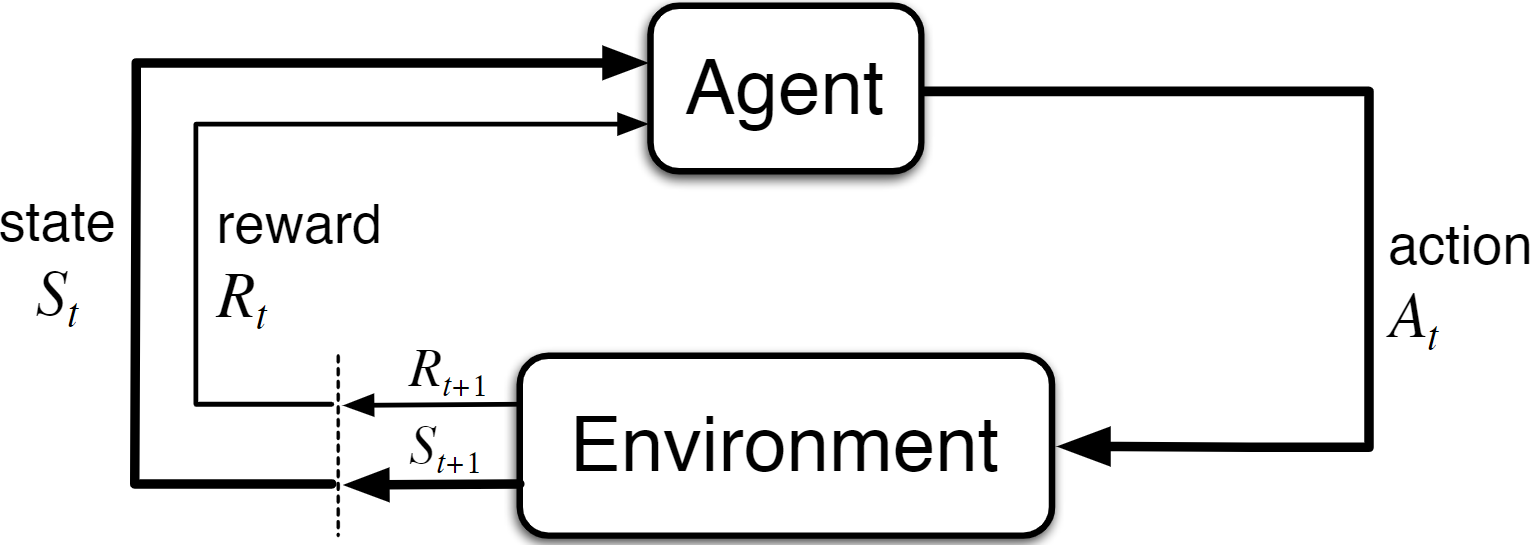
\includegraphics[scale=0.25]{source/images/rl_interaction}%
\caption[Agent-environment loop MDP]{The agent-environment loop can be formalized as a Markov Decision Process. Source: Reprinted from \cite[p.48]{richardsutton2018}}%
\label{fig:rl_interaction}%
\end{figure}

This kind of problem is referred to as finite Markov Decision Process, or finite MDP in short. It can be formalized as a tuple \(\langle \mathcal{S, A, P, R, } \gamma \rangle\), where \(\mathcal{S}\) and \(\mathcal{A}\) are finite sets of states and actions, respectively. \(\mathcal{P}\) is a state transition probability matrix, formalized in \ref{eq:p_transprob}, \(\mathcal{R}\) is a reward function, formalized in \ref{eq:rewfunc}, and \(\gamma\) is a discount factor \(\gamma \in [0,1]\) \cite{silver2020MDP}.
\begin{equation}
\mathcal{P}_{ss'}^{a} = P[S_{t+1} = s' | S_{t} = s, A_{t} = a]
\label{eq:p_transprob}
\end{equation}
\myequations{State transition probability matrix}
\begin{equation}
\mathcal{R}_{s}^{a} = E[R_{t+1} | S_{t} = s, A_{t} = a] 
\label{eq:rewfunc}
\end{equation}
\myequations{Reward function}
Due to the fact that there is no information about \(\mathcal{P}\) and \(\mathcal{R}\) in the Atari environments, see \ref{sec:arcgames}, the agents have to learn from experience to solve the underlying MDP. The discount factor \(\gamma\) is used to compute the weighting of the immediate reward against distant future reward. In addition, it is mathematically convenient and helps with the convergence of the sum in continuous environments and very long episodes. The \textit{return} \(G_{t}\) is the discounted sum of immediate rewards from timestep \textit{t} onwards \ref{eq:returng}.
\begin{equation}
G_{t} = R_{t+1} + \gamma R_{t+2} + \dots =   \displaystyle\sum_{k=0}^{\infty} \gamma ^{k}R_{t+k+1}
\label{eq:returng}
\end{equation}
\myequations{Return function}
A RL agent consists of one or more of the following components. These are a \textit{policy}, a \textit{value function} and a \textit{model} of the environment. The policy directly computes which action is the most optimal one in a given state. The value function estimates the expected return for being in a given state or taking a specific action in a given state. The policy can be seen as the distribution over all actions \textit{A} in a given state \textit{s}. For a specific action \textit{a} it provides the probability of taking action \textit{a} in state \textit{s}:
\begin{equation}
\pi(a|s) = P[A_{t} = a | S_{t} = s]
\label{eq:}
\end{equation}
\myequations{Policy function}
There are two different value functions. The \textit{state}-value function \textit{V} and the \textit{state-action}-value function \textit{Q}, also known as \textit{Q-value} function. They predict how beneficial it is to be in a state and/or to perform a specific action in that state \cite{silver2020RL}. Both value functions behave similar, with the exception that the Q-function keeps values for all actions in a state instead of a single value per state. The state-value function is the expected return \(G_{t}\) starting from state \textit{s}, and then following a policy, see equation \ref{eq:statevalfunc}. The Q-value function is the expected return starting from a state \textit{s}, taking action \textit{a}, and then following the policy, see \ref{eq:qfunc}, \cite{silver2020MDP}.
\begin{equation}
v_{\pi}(s)=E_{\pi}[R_{t+1}+\gamma v_{\pi}(S_{t+1})|S_{t}=s]
\label{eq:statevalfunc}
\end{equation}
\myequations{State-value function}
\begin{equation}
q_{\pi}(s,a) = E_{\pi} [R_{t+1} + \gamma q_{\pi}(S_{t+1}, A_{t+1}) | S_{t} = s, A_{t} = a]
\label{eq:qfunc}
\end{equation} 
\myequations{Q-value function}

In circumstances, where the state space is much smaller compared to the Atari environments', it is sufficient to use a lookup table to store Q-values for every possible state-action pair \cite[p.9]{richardsutton2018}. However, since every single different pixel is representing a new state in Atari environments, it is necessary to approximate the Q-value function. Therefore, the agents \nameref{ssec:dqn}, \nameref{ssec:rain} and \nameref{ssec:apex} make use of deep artificial neural networks (DNN), specifically a deep convolutional artificial neural network (CNN), to approximate Q-functions \cite{2013arXiv1312.5602M, 2017arXiv171002298H, 2018arXiv180300933H}.

\subsection[head={DQN}, tocentry={Deep Q-Network}, reference={DQN}]{Deep Q-Network} \label{ssec:dqn}
The Deep Q-Learning (DQN) agent by \citeA{2013arXiv1312.5602M}, learned to play Atari games by processing game frames of the size 210 x 160 pixel images with a 128-color palette. Due to computational and architectural considerations the original screens where downscaled to 84 x 84 pixel images \cite{Krizhevsky2012}. Because the environment is not fully observable by just one frame, four of the most recent ones are stacked which results in an input with a dimension of  84 x 84 x 4. This input is fed into the architecture seen in figure \ref{fig:dqn_arch} \cite{2013arXiv1312.5602M}. 
\begin{figure}[H]%
\centering
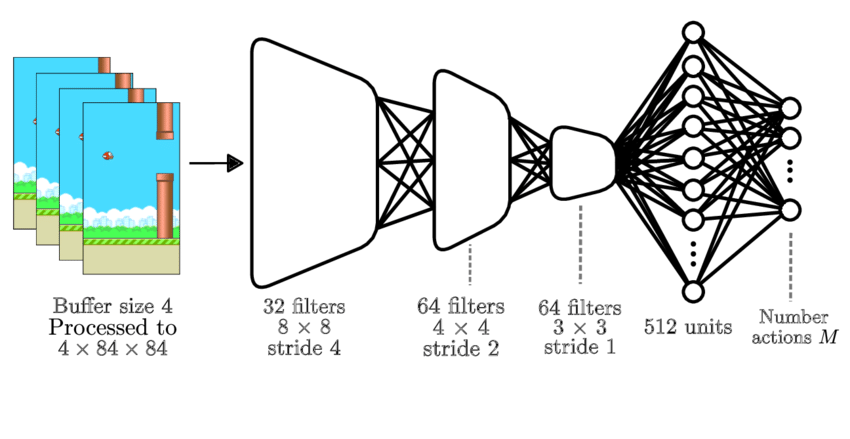
\includegraphics[scale=0.35]{source/images/dqn_arch}%
\caption[DQN Architecture]{DQN Architecture. The use of CNNs for image processing is a well-established standard as illustrated by \protect\cite{LeCun2015}. By only giving the state representation (84 x 84 x 4 images) as an input, the architecture is able to compute Q-values for all possible actions \protect\cite{2013arXiv1312.5602M}. Source: Reprinted from \protect\cite{2017arXiv170104143B}}%
\label{fig:dqn_arch}%
\end{figure}
DQN agents are trained with the back then novel techniques experience replay and fixed Q-targets. Experience replay is a mechanism that stores the experience of an agent at each time step in a replay memory. The advantages of this mechanism are that it reduces variance of updates and increases stability. The reasons for this are that successive updates are no longer related to each other and the removal of dependence of successive experiences on the weights. The benefit of fixed Q-targets is that it improves stability by not changing the weights of the target network for a certain period. During this period, the weights in the Q-network are trained. Eventually, the target network is updated with the new weights of the Q-network \cite[p. 440]{richardsutton2018}. This leads to more stable training and is formalized  by the following loss function equation, that is optimized with stochastic gradient descent \cite{Mnih2015}:
\begin{equation}
L_{i} (\theta _{i}) = E_{(s,a,r,s')\sim U(D)} \Bigg[\bigg(    r+\gamma \max_{a'} Q(s',a';\theta_{i}^{-}-Q(s,a;\theta_{i} \bigg)^2\Bigg]
\label{eq:dqnlossfnc}
\end{equation}
\myequations{Loss function DQN}

\paragraph{Rainbow} \label{ssec:rain}
Rainbow is an improved version of DQN. Six extensions, that all focus on distinct shortcomings, were added to improve the overall performance of DQN. These are Double Q-learning, Prioritized replay, Dueling networks, Multi-step learning, Distributional RL and Noisy Nets.
\subparagraph{Double Q-learning}
In Double Q-learning the action selection is decoupled from its evaluation in order to address the issue of overestimating specific actions which leads to biased updates otherwise.
\subparagraph{Prioritized replay}
In normal experience replay, transitions are sampled uniformly regardless of their significance. With this method, transitions are chosen based on their learning potential, computed by the \textit{TD error}.
\subparagraph{Dueling networks}
The Q-function is split after the convolution layers. Two separate estimators, state value function and advantage function, see section \ref{ssec:a2c}, are used to generalize states and actions independently, without changing the fundamental algorithm.
\subparagraph{Multi-step learning}
Rather than computing the target value based on only the current reward, rewards from multiple steps are accumulated, which leads to faster learning.
\subparagraph{Distributional RL}
Instead of learning the expected return, the agent learns to approximate the distribution of returns.
\subparagraph{Noisy Nets}
In DQN an \(\epsilon\)-greedy strategy, the probability to take a random action, is used for exploration of the environment. In this extension noise is added to the network weights for better exploration \cite{2017arXiv171002298H}.

\paragraph{Ape-X} \label{ssec:apex}
Ape-X is a distributed architecture, where actor and learner are decoupled. 
\begin{figure}[H]%
\centering
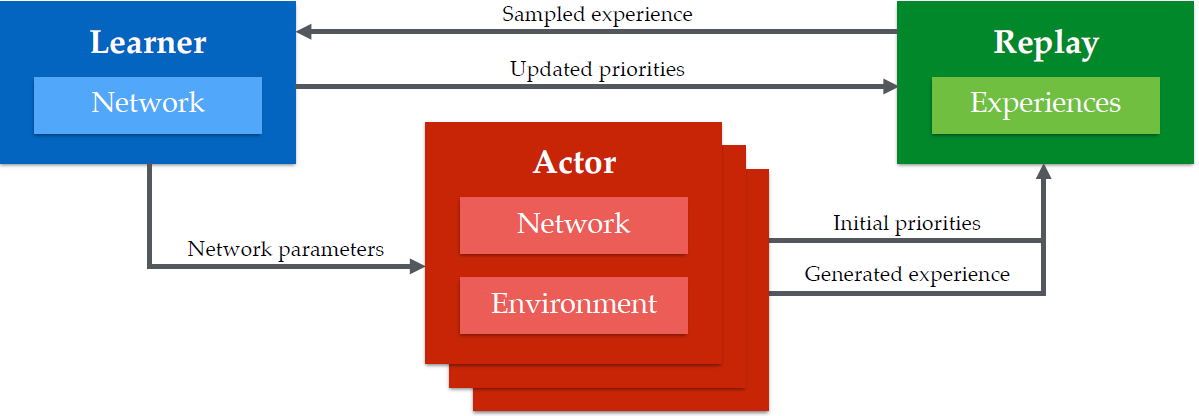
\includegraphics[scale=0.35]{source/images/apex_arch}%
\caption[Ape-X architecture]{Ape-X architecture. Source: Reprinted from \protect\cite{2018arXiv180300933H}}%
\label{fig:apex_arch}%
\end{figure}
Multiple actors interact in parallel with their own environment instance to generate experience, which is then saved in a shared prioritized experience replay, as seen in figure \ref{fig:apex_arch}. The learner updates the network by sampling the replays \cite{2018arXiv180300933H}.

\subsection[head={A2C}, tocentry={Advantage Actor Critic}, reference={A2C}]{Advantage Actor Critic} \label{ssec:a2c}
In the Advantage Actor Critic algorithm (A2C) there is an actor, that controls the actions of an agent and a critic that measures the expected return of those actions. A parametrized policy, \(\pi_{\theta}(a|s)\), operates as the actor and a parametrized value function, \(V(s_{t};\theta_{v})\), is used as the critic. In contrast to \nameref{ssec:dqn}, this algorithm uses two components, policy and value function, rather than one. The A2C is a policy gradient variant that is optimized by the following objective function: 
\begin{equation}
\nabla_{\theta}J(\theta)=E_{\pi_{\theta}}[\nabla_{\theta}log\pi_{\theta}(s,a) A^{w}(s,a)]
\label{eq:a2c}
\end{equation}
\myequations{A2C objective function}
Both, the actor and critic, have their own set of parameters, \(\theta\) and \textit{w}, respectively. The actor listens to suggestions from the critic and updates \(\theta\) accordingly. The A2C uses the advantage function as its actor. That function can significantly reduce variance of policy gradient and is formalized by:
\begin{equation}
A(s,a)=Q_{w}(s,a)-V_{v}(s)
\label{eq:advfunc}
\end{equation}
\myequations{Advanced function}
In this formalization, two set of parameters, \textit{w} and \textit{v}, are required for approximating the value functions. However, this leads to a total of three sets of parameters, or networks, together with the parameters \(\theta\) of the policy network. Optimizing three sets of parameters jointly is computationally expensive and hard. Therefore, the TD error of the state-value function, formalized by \ref{eq:errstateval}, is used, to estimate the advantage function and reduce the set of parameters for the advantage function to one \cite{2016arXiv160201783M}.
\begin{equation}
\delta_{v}=r+\gamma V_{v}(s')-V_{v}(s)
\label{eq:errstateval}
\end{equation}
\myequations{TD error of state-value function}

\section{Evolutionary Algorithm}

\subsection[head={GA}, tocentry={Genetic Algorithms}, reference={GA}]{Genetic Algorithms} \label{ssec:ga}
The genetic algorithm (GA) used by \cite{2017arXiv171206567P} is an non-gradient-based alternative, to the previously mentioned RL algorithms, for DNNs. The populations that are used in the GA algorithm include a variable amount of \textit{N} individuals. Individuals, or genotypes, are represented as different parameter vectors \(\theta\) of a deep neural network. During the evolution of the population, in every \textit{generation} the genotypes are evaluated based on their \textit{fitness}, which is the reward from the Atari environment. After every generation, the top individuals are selected as the parents for the next generation. To generate the next generation, a process, where a parent is \textit{mutated} by applying additive Gaussian noise to the genotype, is repeated for \textit{N-1} times. A technique called \textit{elitism}, where the best individual from the previous generation is copies unmodified, is applied to the \(N^{th}\) individual. Due to memory and network transmission costs, the neural networks are not stored in variables, rather the seeds of the random number generator, that is used to initialize the network and evolve the weights of the network, are used to reproduce the network.

\subsection[head={ES}, tocentry={Evolution Strategies}, reference={ES}]{Evolution Strategies} \label{ssec:es}
Evolution strategies (ES) is another alternative to the RL algorithms. It is different from \nameref{ssec:ga}, because it performs stochastic gradient ascent on the parameters instead of evolution. \cite{2017arXiv171206567P}. The ES is a black box optimization technique, which means that the algorithm has no direct access to the gradient of the function that is being optimized. This leads to the setup, where the ES algorithm takes the parameters of the policy network as its input and produces a single output. The algorithm is perturbing the policy parameters with a sample of gaussian noise parameters and computes the return \(G_{t}\) for the perturbed parameters. Finally, the results of multiple runs are combined and the initial parameters are updated with the weighted sum of noise vectors depending on the return they produced during the test \cite{2017arXiv170303864S}. The gradient estimator that is used in this procedure is formalized by:
\begin{equation}
\nabla_{\theta}E_{\epsilon\sim N(0,I)}G(\theta+\sigma\epsilon)=\frac{1}{\sigma}E_{\epsilon\sim N(0,I)}\{G(\theta+\sigma\epsilon)\epsilon\}
\label{eq:esalgo}
\end{equation}
\myequations{EA Gradient estimator function}

